\documentclass[conf]{new-aiaa}
% Replace your main .tex file with this source in the existing AIAA project.
% Upload the supplied figures folder and retain your existing new-aiaa.cls.
\usepackage[utf8]{inputenc}
\usepackage[T1]{fontenc}
\usepackage{graphicx}
\usepackage{amsmath}
\usepackage{tabularx,booktabs}
\usepackage{url}
\urlstyle{same}
\usepackage{placeins}
\graphicspath{{figures/}}
\hypersetup{hidelinks,pdftitle={Effect of Orbital Altitude on Satellite Revisit Time over Central Europe},pdfauthor={Danillo Kruppel}}
\title{Effect of Orbital Altitude on Satellite Revisit Time over Central Europe}
\author{Danillo Kr\"uppel}
\affil{Space Systems Engineer, AiShed Consulting}

\begin{document}
\maketitle

\begin{abstract}
This study compares geometric Earth-observation access over Central Europe
for four initially circular satellite orbits at nominal altitudes of 400,
500, 600, and 700 km. Thirty-day GMAT trajectories are analysed over an
800-point geographic grid using an idealised nadir-pointing sensor with a
fixed 20-degree half-angle. The regional area-weighted mean of per-target
mean revisit gaps is 42.86, 28.51, 29.96, and 26.30 h, respectively. Average
daily coverage increases from 46.98\% at 400 km to 68.48\% at 700 km. However,
the largest observed complete gap is shortest at 600 km, at 88.20 h,
compared with 111.45 h at 700 km and 420.12 h at 500 km. These differences
show that mean performance and worst observed interruption favour different
altitudes. Geometry checks and a 20-second coarsening diagnostic support
initial assessment of the analysis, but do not establish fine-step
convergence. The results are preliminary, configuration-specific estimates;
finer temporal and geographic sampling and additional initial-geometry
cases are required before a final mission-design recommendation.
\end{abstract}

\section{Introduction}
\label{sec:introduction}
Earth-observation mission design requires a relationship to be established
between the information sought on the ground and the opportunities available
from orbit. For a regional monitoring mission, the ability to observe a
location once is insufficient to describe its usefulness: the time between
successive opportunities is also relevant. Revisit performance therefore
provides a means of comparing orbital configurations against a temporal
observation objective. Coverage studies must nevertheless distinguish an
opportunity to view a target from the acquisition of a usable image. The
former follows from orbital and sensor geometry, whereas the latter may
also depend on illumination, cloud cover, instrument performance, and
operational scheduling.

Professional mission studies treat coverage as a coupled orbit--instrument
problem. Nag et al.~\cite{nag2016} explore Earth-imaging constellation
architectures using orbital and instrument variables, evaluate temporal
coverage metrics, and compare results with an independent analysis system.
Their work provides a methodological precedent for defining design
variables, computing geographic access, and examining differences between
implementations. A complementary lesson is that simulation output requires
explicit supporting evidence. Hughes et al.~\cite{hughes2014} describe the
verification and validation of GMAT using independent reference tools and
comparison tests. These examples motivate a study in which performance
comparisons and checks on the analysis method are developed together.

The present study narrows the design space to one satellite and four
candidate initial altitudes. Increasing altitude changes the orbital period
and, for a fixed angular field of view, the sensor footprint. The resulting
revisit performance also depends on the ground-track pattern, target
latitude, and selected orbital orientation. A comparison based only on the
number of daily revolutions would therefore omit the geometry that
determines whether a target is observable. The research question is how
altitude affects mean and maximum geometric revisit gaps over Central
Europe when nominal inclination and sensor angular field of view are held
fixed. The contribution is a reproducible regional comparison and an
explicit account of its numerical limitations, rather than a new
coverage algorithm.

The completed baseline combines GMAT propagation with Python processing of
time-tagged Earth-fixed spacecraft positions. All cases use the same
30-day interval, target grid, and sensor model. Alongside regional mean
performance, the comparison examines the largest complete gap and its
geographic distribution. A coarsening diagnostic evaluates the effect of
retaining every other trajectory sample; finer-step and initial-geometry
campaigns remain future work. Dividing the computation between a propagation
tool and an analysis driver follows an established engineering workflow:
Nickel et al.~\cite{nickel2016}, for example, describe automated GMAT--MATLAB
simulations for the TESS mission. Cloud cover, imaging task scheduling, and
downlink capacity remain outside the present baseline.

Section~\ref{sec:definition} defines the observation study.
Section~\ref{sec:method} presents the geometry and metrics.
Section~\ref{sec:verification} reports completed checks and outstanding
verification work. Section~\ref{sec:results} discusses the numerical
comparison, followed by the conclusions in Section~\ref{sec:conclusion}.

\section{Study Definition}
\label{sec:definition}
\subsection{Region and Target Grid}
The region of interest is a user-defined rectangle spanning
$5^{\circ}$--$25^{\circ}$ east longitude and
$45^{\circ}$--$55^{\circ}$ north geodetic latitude. This explicit boundary
is used as a practical Central European study area, rather than as an
official geographic definition. Both land and water within the rectangle
are retained. Country boundaries provide map context only.

The rectangle is divided into $0.5^{\circ}\times0.5^{\circ}$ cells. Their
centres define 40 longitude values and 20 latitude values, giving 800
targets. Longitudes run from $5.25^{\circ}$ to $24.75^{\circ}$ east and
latitudes from $45.25^{\circ}$ to $54.75^{\circ}$ north. Targets lie at zero
height on the WGS~84 ellipsoid. Figure~\ref{fig:region} shows the grid.
A cell is represented by its centre point; observing the point does not
imply that the whole cell has been imaged.

\begin{figure}[htbp]
\centering
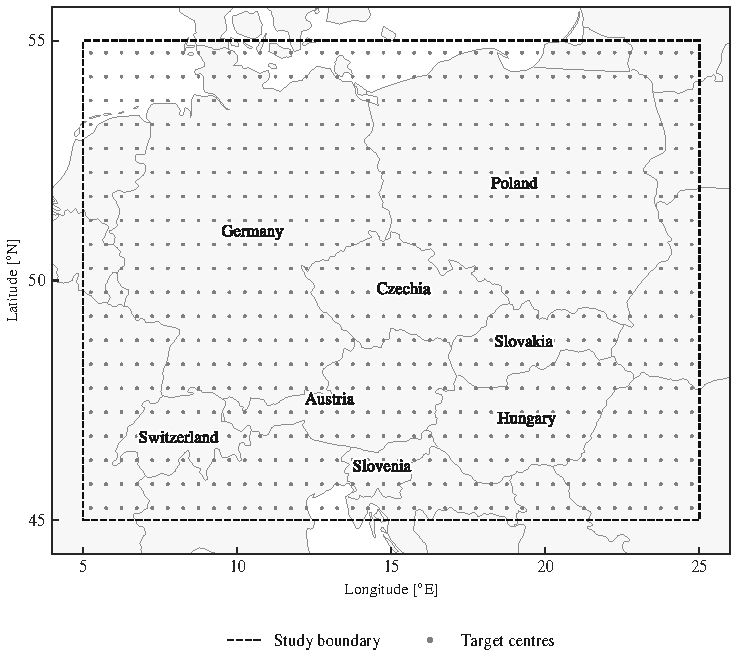
\includegraphics[width=0.86\linewidth]{target_region.pdf}
\caption{Rectangular study region and the 800 target locations. The grid
includes land and water. Country boundaries: Natural Earth.}
\label{fig:region}
\end{figure}

\subsection{Orbit Cases and Observation Concept}
Four trajectories were generated for nominal initial altitudes of 400,
500, 600, and 700 km. The common setup specifies an initially circular
orbit at $60^{\circ}$ inclination, with right ascension of the ascending
node, argument of perigee, and true anomaly set to zero in the initial
EarthMJ2000Eq representation. For a circular orbit, the sum of the last
two angles defines the initial argument of latitude. No sun-synchronous
condition is imposed.

The initial semi-major axes are 6778.137, 6878.137, 6978.137, and 7078.137 km,
using 6378.137 km as the reference radius for the altitude labels. These
labels describe the initial configuration, rather than a constant height
above an oblate Earth throughout propagation. The common interval extends
from 1 January 2026 at 00:00 UTC to 31 January 2026 at 00:00 UTC.

An idealised circular conical sensor points towards Earth's centre, with
half-angle $\alpha=20^{\circ}$ and full angular field of view $40^{\circ}$.
There is no off-nadir steering. Its boresight is geocentric nadir, which is
distinct from the local ellipsoid normal. Geometric access requires a target
to lie inside the cone and to have an unobstructed line of sight.
No daylight or cloud filter is applied, so night-time opportunities are
included. The sensor is a modelling assumption, not a selected instrument.

\begin{table}[htbp]
\caption{Baseline analysis definition and trajectory-input record.}
\label{tab:configuration}
\centering
\begin{tabularx}{\linewidth}{@{}p{0.35\linewidth}X@{}}
\toprule
Parameter & Value \\
\midrule
Nominal initial altitude & 400, 500, 600, 700 km \\
Nominal initial eccentricity / inclination & 0 / $60^{\circ}$ \\
Nominal initial RAAN / argument of latitude & $0^{\circ}$ / $0^{\circ}$ \\
Common UTC interval & 1--31 January 2026, 30 days \\
Exported position frame / units & GMAT EarthFixed / km \\
Samples per trajectory & 259,201, including both endpoints \\
Output spacing & Approximately 10 s \\
Sensor half-angle / pointing & $20^{\circ}$ / towards Earth's centre \\
Target geometry & Zero-height WGS~84 ellipsoid \\
Region / target count & $5$--$25^{\circ}$E, $45$--$55^{\circ}$N / 800 \\
Illumination, clouds, scheduling & Not modelled \\
\bottomrule
\end{tabularx}
\end{table}

The analysis verifies timestamps, frames and initial position radii directly
from the CSVs. The complete initial-state and force-model definitions must
also be retained in the original GMAT scripts for full reproducibility;
the CSV exports alone do not identify the force model or integrator.

\section{Analysis Method}
\label{sec:method}
Figure~\ref{fig:workflow} links the common observation assumptions and the
four trajectories to the reported coverage and revisit measures. The
calculation is applied independently to each altitude with identical target
and sensor definitions.

\begin{figure}[htbp]
\centering
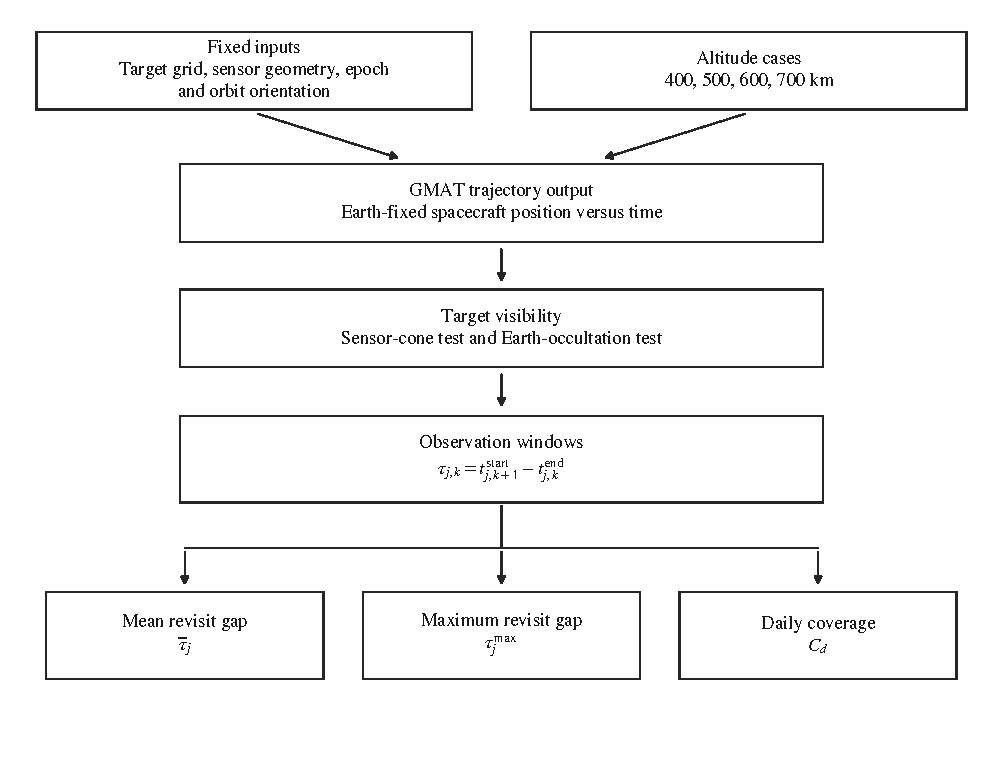
\includegraphics[width=0.86\linewidth,height=0.76\textheight,keepaspectratio]{analysis_workflow.pdf}
\caption{Analysis structure linking altitude-dependent trajectories to
observation windows and performance measures. The equation defines revisit gap as the interval from the end of one
observation window to the start of the next.}
\label{fig:workflow}
\end{figure}

\subsection{Trajectory Inputs and Earth Geometry}
The input record contains elapsed seconds, A1 modified Julian epoch,
A1 Gregorian date, and spacecraft EarthFixed Cartesian coordinates.
All four files contain matching sample times from 0 to 2,592,000 s.
Absolute A1 epochs are retained for consistency checks; daily bins are
formed from elapsed seconds referenced to the common UTC start. A1 dates
are not interpreted as UTC dates.

Ground coordinates are converted to Earth-fixed Cartesian positions using
WGS~84 semi-major axis $a_E=6378.137$ km and flattening
$f=1/298.257223563$, as specified by NGA~\cite{wgs84}. With
$e_E^2=f(2-f)$ and geodetic latitude and longitude $(\phi_j,\lambda_j)$,
\begin{equation}
N_j=\frac{a_E}{\sqrt{1-e_E^2\sin^2\phi_j}},\qquad
\mathbf{g}_j=\begin{bmatrix}
N_j\cos\phi_j\cos\lambda_j\\
N_j\cos\phi_j\sin\lambda_j\\
N_j(1-e_E^2)\sin\phi_j
\end{bmatrix}.
\label{eq:ground}
\end{equation}
Here $\mathbf{g}_j$ is the zero-height target position. The outward unit
normal is
\begin{equation}
\mathbf{n}_j=\begin{bmatrix}
\cos\phi_j\cos\lambda_j\\
\cos\phi_j\sin\lambda_j\\
\sin\phi_j
\end{bmatrix}.
\label{eq:normal}
\end{equation}

\subsection{Visibility and Observation Windows}
For spacecraft position $\mathbf{r}(t)$, the sensor boresight and
spacecraft-to-target unit vector are
\begin{equation}
\mathbf{b}(t)=-\frac{\mathbf{r}(t)}{\|\mathbf{r}(t)\|},\qquad
\mathbf{u}_j(t)=\frac{\mathbf{g}_j-\mathbf{r}(t)}{\|\mathbf{g}_j-\mathbf{r}(t)\|}.
\end{equation}
A sample is visible when both conditions hold:
\begin{equation}
\mathbf{b}(t)\cdot\mathbf{u}_j(t)\geq\cos\alpha,
\qquad [\mathbf{r}(t)-\mathbf{g}_j]\cdot\mathbf{n}_j>0.
\label{eq:visible}
\end{equation}
The first condition applies the sensor cone. The second is the horizon
condition for a target on a convex ellipsoid, excluding lines of sight
through Earth. Terrain and atmospheric refraction are omitted.

Consecutive visible samples are grouped into observation windows. At an
internal transition, the window boundary is estimated at the midpoint
between the visible and invisible sample times. A window touching the
analysis endpoint is clipped there and flagged. This procedure approximates
boundary timing; it does not solve continuous-time access events and can
miss a sufficiently short window between output samples.

For target $j$, with $K_j$ windows, the complete gap between windows $k$ and
$k+1$ is
\begin{equation}
\tau_{j,k}=t^{\mathrm{start}}_{j,k+1}-t^{\mathrm{end}}_{j,k},
\qquad k=1,\ldots,K_j-1.
\label{eq:gap}
\end{equation}
Leading and trailing unobserved portions of the 30-day interval are
boundary-censored. They are stored separately and excluded from the set of
complete gaps. A target with fewer than two windows receives no mean or
maximum complete-gap estimate, rather than a zero value.

\subsection{Revisit and Coverage Metrics}
For targets with at least two windows, the mean and maximum complete gaps are
\begin{equation}
\bar{\tau}_j=\frac{1}{K_j-1}\sum_{k=1}^{K_j-1}\tau_{j,k},\qquad
\tau^{\max}_j=\max_k\tau_{j,k}.
\end{equation}
Regional summaries use approximate spherical cell-area weights. For a cell
with longitude width $\Delta\lambda_j$ and latitude edges
$\phi_j^-,\phi_j^+$,
\begin{equation}
\widetilde{w}_j=\Delta\lambda_j(\sin\phi_j^+-\sin\phi_j^-),\qquad
w_j=\frac{\widetilde{w}_j}{\sum_l\widetilde{w}_l}.
\end{equation}
Angular quantities in this expression are in radians. These weights
compensate for unequal latitude--longitude cell areas, but are not exact
ellipsoidal areas. The regional mean is
\begin{equation}
\bar{\tau}_{R}=\sum_j w_j\bar{\tau}_j,
\qquad \tau_R^{\max}=\max_j\tau_j^{\max}.
\label{eq:regional}
\end{equation}
Equation~\eqref{eq:regional} averages per-target means, not all individual
gaps pooled across the region. All 800 targets have complete gaps in the
baseline. If estimates are missing, the implementation renormalises the
mean over available targets and separately reports the excluded area.

Daily coverage $C_d$ is the weighted fraction of targets with a nonzero-duration
observation window overlapping day $d$:
\begin{equation}
C_d=100\sum_jw_j I_{j,d},\qquad
\bar C=\frac{1}{30}\sum_{d=1}^{30}C_d.
\end{equation}
Here $I_{j,d}$ is one if such a window exists and zero otherwise. Each day
is a 24-hour bin from the common start epoch. Coverage refers to sampled
target points and is an approximation of observed regional area.

\subsection{Implementation and Reproducibility}
The Python calculation evaluates visibility in chunks, groups samples by
target, and exports per-target statistics, observation-window tables, daily
coverage, and regional summaries. The recorded run uses Python 3.12.14,
NumPy 2.3.5, and Matplotlib 3.10.8; GeoPandas is used for country-boundary
plots. The metadata records input SHA-256 hashes, the observation model,
software versions, and trajectory checks. Natural Earth boundaries are
used for cartographic context~\cite{naturalearth}.

\section{Verification and Sampling Diagnostic}
\label{sec:verification}
\subsection{Completed Input and Geometry Checks}
All trajectories span the same 30 days, with 259,201 finite samples,
strictly increasing elapsed times, and matching absolute initial epochs.
Their initial Earth-centred radii agree with the four nominal semi-major
axes in Table~\ref{tab:configuration}. Exported variables are spacecraft
positions in EarthFixed, rather than Earth's position in that frame.

The vectorised visibility test was compared with a direct implementation
of the boresight/line-of-sight dot product and surface-normal horizon test.
Known nadir and antipodal cases were checked. An analytic equatorial
footprint boundary supplied a further test: on the equator the WGS~84
section is a circle, and, for an off-nadir half-angle below the apparent
limb, the footprint half-width in geocentric angle is
\begin{equation}
\psi=\sin^{-1}\!\left(\frac{r}{a_E}\sin\alpha\right)-\alpha.
\end{equation}
Targets just inside and outside that boundary were classified as expected.
An additional direct-vector comparison at 1,000 distributed epochs for the
largest-gap 500 km target agreed with the vectorised result. These checks
address implementation consistency; they do not independently validate the
full propagated mission or establish access-event timing accuracy.

\subsection{Ten-Second Versus Twenty-Second Sampling}
The baseline uses the approximately 10-second output. A second calculation
retains every other sample, producing a 20-second series without rerunning
GMAT. Table~\ref{tab:coarsening} and Fig.~\ref{fig:sampling} report the changes.
The regional mean gap increases by 0.78--2.89\%, and mean daily coverage
falls by 0.36--1.15 percentage points. At 400 km, the largest observed gap
increases from 172.79 to 183.02 h, a 5.92\% change.

\begin{table}[htbp]
\caption{Coarsening diagnostic. Changes are relative to the 10-second baseline.}
\label{tab:coarsening}
\centering
\small
\begin{tabular}{@{}rrrr@{}}
\toprule
Altitude (km) & Mean-gap change (\%) & Coverage change (pp) & 20 s largest gap (h)\\
\midrule
400 & +2.89 & -1.15 & 183.02\\
500 & +1.21 & -0.62 & 420.12\\
600 & +1.25 & -0.56 & 88.21\\
700 & +0.78 & -0.36 & 111.45\\
\bottomrule
\end{tabular}
\end{table}

\begin{figure}[htbp]
\centering
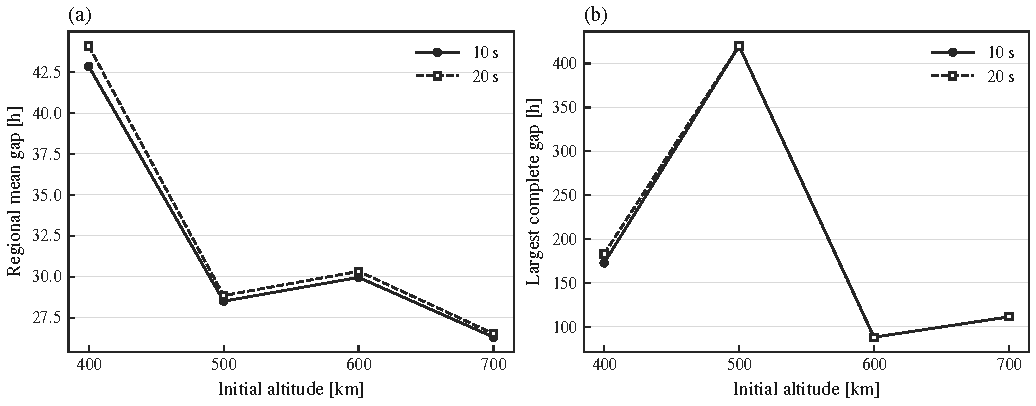
\includegraphics[width=\linewidth]{sampling_diagnostic.pdf}
\caption{Revisit metrics from 10-second samples and a 20-second subsample.
This is a coarsening diagnostic, not evidence of convergence towards a
finer-step solution.}
\label{fig:sampling}
\end{figure}

The regional-mean and largest-gap altitude rankings are unchanged under this
coarsening. However, short windows may be missed at both resolutions, and
stable rankings do not bound numerical error. Native GMAT output at 5 s or
finer, a finer target grid, extended durations, and different initial orbital
orientations have not yet been analysed.

\section{Results and Discussion}
\label{sec:results}
\subsection{Regional Performance and Altitude Trade-Off}
Table~\ref{tab:results} summarises the 10-second baseline. All 800 targets
have at least two observation windows in every altitude case, so the mean
includes the whole sampled region. The area-weighted mean gap falls from
42.86 h at 400 km to 26.30 h at 700 km, a 38.62\% reduction. The trend is
not monotonic: the 600 km mean gap, 29.96 h, exceeds the 500 km value of
28.51 h. Average daily coverage increases monotonically across these four
cases, from 46.98\% to 68.48\%, an increase of 21.50 percentage points.

\begin{table}[htbp]
\caption{Preliminary 30-day geometric-access results at approximately 10-second sampling.}
\label{tab:results}
\centering
\begin{tabular}{@{}rrrrr@{}}
\toprule
Altitude & Regional mean & Largest complete & Mean daily & Min. daily\\
(km) & gap (h) & gap (h) & coverage (\%) & coverage (\%)\\
\midrule
400 & 42.86 & 172.79 & 46.98 & 43.18\\
500 & 28.51 & 420.12 & 54.36 & 50.76\\
600 & 29.96 & 88.20 & 61.67 & 55.24\\
700 & 26.30 & 111.45 & 68.48 & 55.33\\
\bottomrule
\end{tabular}
\end{table}

\begin{figure}[htbp]
\centering
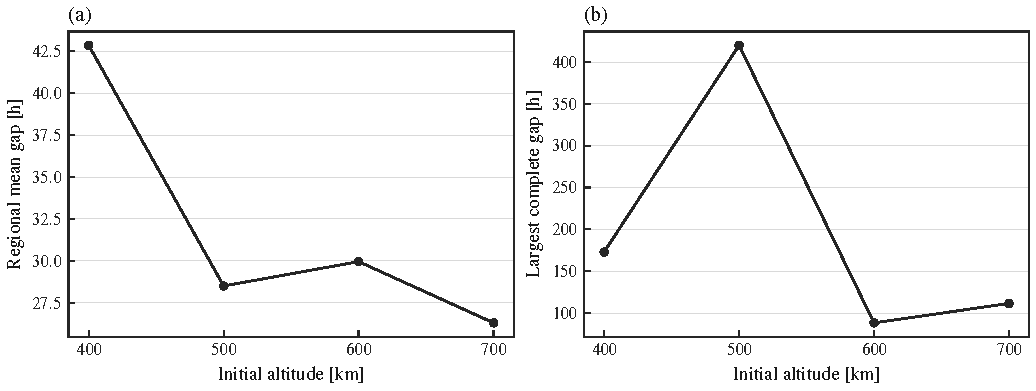
\includegraphics[width=\linewidth]{altitude_revisit.pdf}
\caption{Regional mean of per-target mean gaps (left) and largest observed
complete gap across the grid (right). The two measures favour different
altitudes.}
\label{fig:altitude}
\end{figure}

The 700 km case is strongest on regional mean gap and average daily
coverage, whereas 600 km gives the smallest largest observed gap, 88.20 h.
The 500 km case has the longest complete interruption, 420.12 h
(approximately 17.51 days), despite its relatively favourable regional mean.
Thus a selection based only on the regional mean would omit a material
aspect of service continuity. The reported maxima are the longest complete
gaps observed in this interval, not guaranteed bounds on future performance.

\subsection{Geographic Distribution and Long-Gap Locations}
Figure~\ref{fig:maps} maps the per-target mean gaps with one common scale.
At 400 km, mean gaps generally increase towards the southern part of the
region. The 700 km distribution is lower overall, while the 500 km case
shows pronounced spatial structure. These results support reporting
geographic detail alongside a single regional average.

\begin{figure}[htbp]
\centering
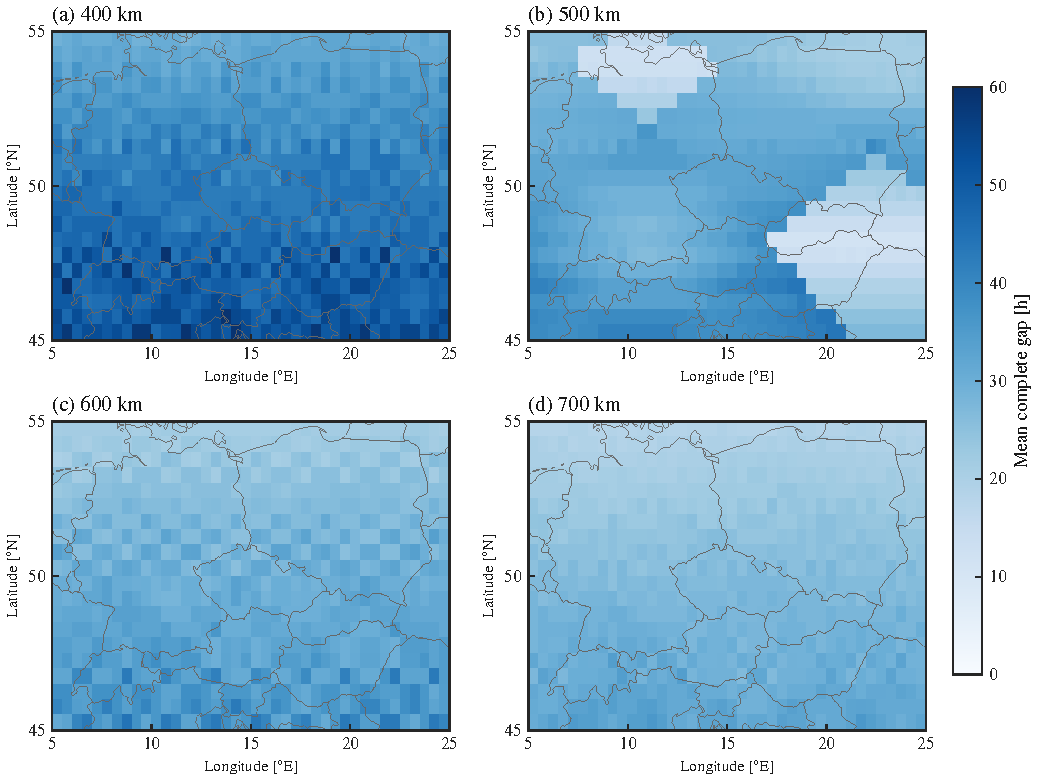
\includegraphics[width=\linewidth,height=0.75\textheight,keepaspectratio]{revisit_maps.pdf}
\caption{Per-target mean complete revisit gap. The same colour scale is used
in all panels. Each cell is represented by its centre target; country
boundaries are supplied by Natural Earth.}
\label{fig:maps}
\end{figure}

The maximum-gap maps in Fig.~\ref{fig:maxmaps} reveal an additional pattern.
The 500 km long gaps affect a spatial band, rather than appearing solely as
one isolated target. One largest-gap target is at $11.75^{\circ}$E,
$48.25^{\circ}$N; its 26 detected windows include the 420.12 h complete gap.
The spatial structure is compatible with altitude-dependent pass geometry,
but a specific resonance or repeat-cycle explanation has not been tested.
The extreme requires finer temporal sampling and inspection of its access
history before it is treated as a robust design result.

\begin{figure}[htbp]
\centering
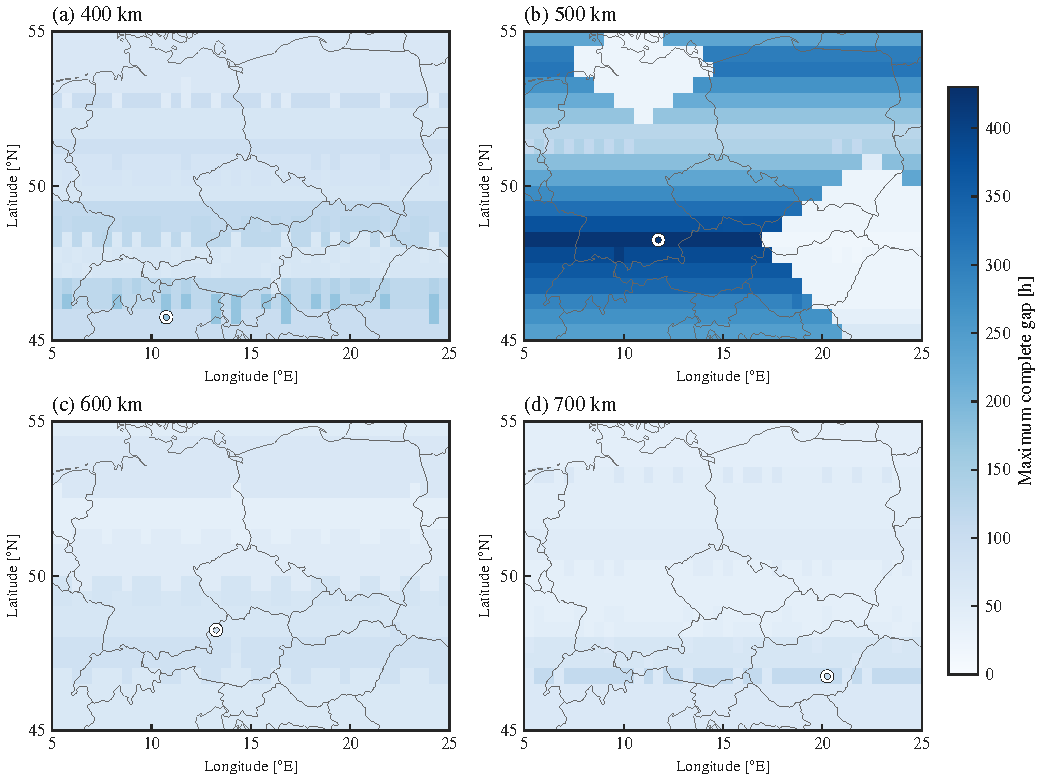
\includegraphics[width=\linewidth,height=0.78\textheight,keepaspectratio]{maximum_gap_maps.pdf}
\caption{Largest observed complete revisit gap at each target. Darker
colours indicate longer interruptions; all panels use a shared scale.
White circles identify one largest-gap target per altitude. Boundary-censored
intervals are excluded. Country boundaries: Natural Earth.}
\label{fig:maxmaps}
\end{figure}

\subsection{Daily Coverage and Distribution of Mean Gaps}
Figure~\ref{fig:daily} shows how coverage changes from day to day. The 700 km
case has the highest 30-day average, but its lowest daily value is 55.33\%,
close to the 600 km minimum of 55.24\%. An average coverage advantage
therefore does not imply an equally large advantage on the least favourable
day. None of the configurations provides full regional coverage on every
day of the sampled interval. This is consistent with the restricted
single-satellite observation concept, and is not a statement about the
performance of a constellation or a steerable instrument.

\begin{figure}[htbp]
\centering
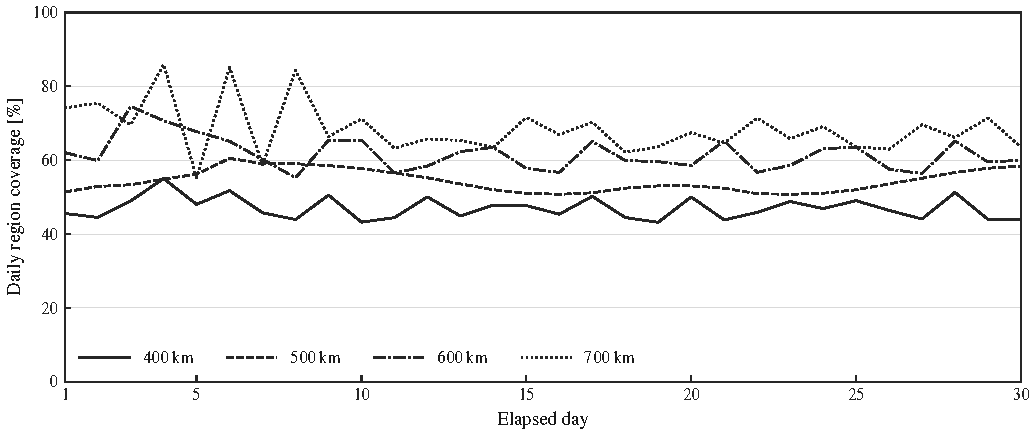
\includegraphics[width=\linewidth]{daily_coverage.pdf}
\caption{Daily area-weighted fraction of targets with at least one
geometric opportunity. Each bin spans 24 hours from the common UTC start;
cloud cover, illumination and image scheduling are excluded.}
\label{fig:daily}
\end{figure}

Figure~\ref{fig:distribution} presents the cumulative area-weighted
distribution of per-target mean gaps. The 700 km curve lies largely to the
left of the others, while 500 and 600 km trade relative performance across
different parts of the distribution. This distribution complements the regional means; it does not describe
the probability of acquiring usable imagery.

\begin{figure}[htbp]
\centering
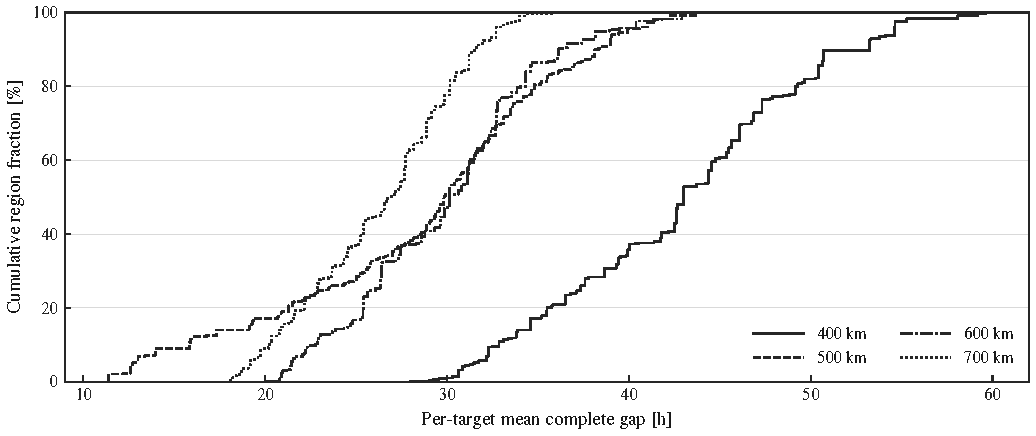
\includegraphics[width=0.90\linewidth]{revisit_distribution.pdf}
\caption{Cumulative region fraction as a function of per-target mean
complete gap. Area weights refer to the full target region; all baseline
targets have defined complete-gap estimates.}
\label{fig:distribution}
\end{figure}

\subsection{Limitations and Remaining Work}
The results depend on the initial epoch and orbital geometry, a fixed
20-degree sensor half-angle, and the chosen regional boundary. The sensor
has no steering or imaging-quality constraint. Coverage includes night-time
and cloudy conditions, and says nothing about data return, ground sampling
distance, battery capacity, or an operational imaging schedule.

Temporal sampling can miss short windows, while midpoint boundary estimates
introduce event-time approximation. Geographic sampling represents cells
by points and has not been refined. The finite interval censors leading and
trailing unobserved periods; excluding them can affect comparisons when
windows cluster in time. A long observed complete gap is therefore useful
evidence about the sampled scenario, but is not a mission-lifetime maximum.
The spherical area weights also approximate ellipsoidal cell areas.

Finally, the exported CSVs do not preserve GMAT's gravity-field truncation,
perturbation selections, integrator settings, or software release. The
intended setup used a simplified Earth-gravity model including $J_2$, with
other perturbations disabled, but these settings have not been audited
against the native scripts. Archiving and checking the four original GMAT
scripts is required before presenting the study as fully reproducible.
These limitations should be resolved through a controlled verification
campaign, rather than by interpreting more decimal places in the existing
summary statistics.

\FloatBarrier
\section{Conclusion}
\label{sec:conclusion}
For the specified single-satellite, 20-degree half-angle observation concept,
nominal altitude changes materially affect regional geometric access.
Across the four sampled configurations, 700 km gives the lowest regional
area-weighted mean complete gap, 26.30 h, and highest average daily coverage,
68.48\%. Relative to 400 km, these represent a 38.62\% reduction in mean gap
and a 21.50 percentage-point increase in average daily coverage. Nevertheless,
mean revisit performance does not improve monotonically with altitude.

A different criterion leads to a different preferred case: 600 km has the
shortest largest observed complete gap, 88.20 h, compared with 111.45 h at
700 km. The 500 km case demonstrates the limitation of average-only
selection, combining a regional mean of 28.51 h with a 420.12 h interruption
at a target in the region. A mission decision must therefore specify
whether typical access, geographic fairness, or avoidance of long gaps is
the controlling requirement. None of these results establishes guaranteed
daily access to the whole region.

The analysis supports a preliminary trade study, not a universal optimum.
Input checks and independent geometry calculations passed, and the
10-to-20-second coarsening retained the altitude rankings; however,
fine-step and grid convergence are unproven. The next steps are to archive
the complete GMAT configurations, rerun with finer output sampling, refine
the target grid, and test initial geometry and duration. Until those checks
are complete, 700 km is the leading candidate for mean access and coverage,
and 600 km for the observed worst-gap criterion, within this scenario only.

\appendix
\section{Supporting Access Visualisations}
\label{sec:appendix}
Figure~\ref{fig:tracks} shows the first-day subsatellite tracks. Its latitude
is geocentric, unlike the geodetic target-grid latitude, and it is used only
for qualitative orientation. Sensor footprints are not shown. It does not
replace the visibility calculation in Eq.~\eqref{eq:visible}.

\begin{figure}[htbp]
\centering
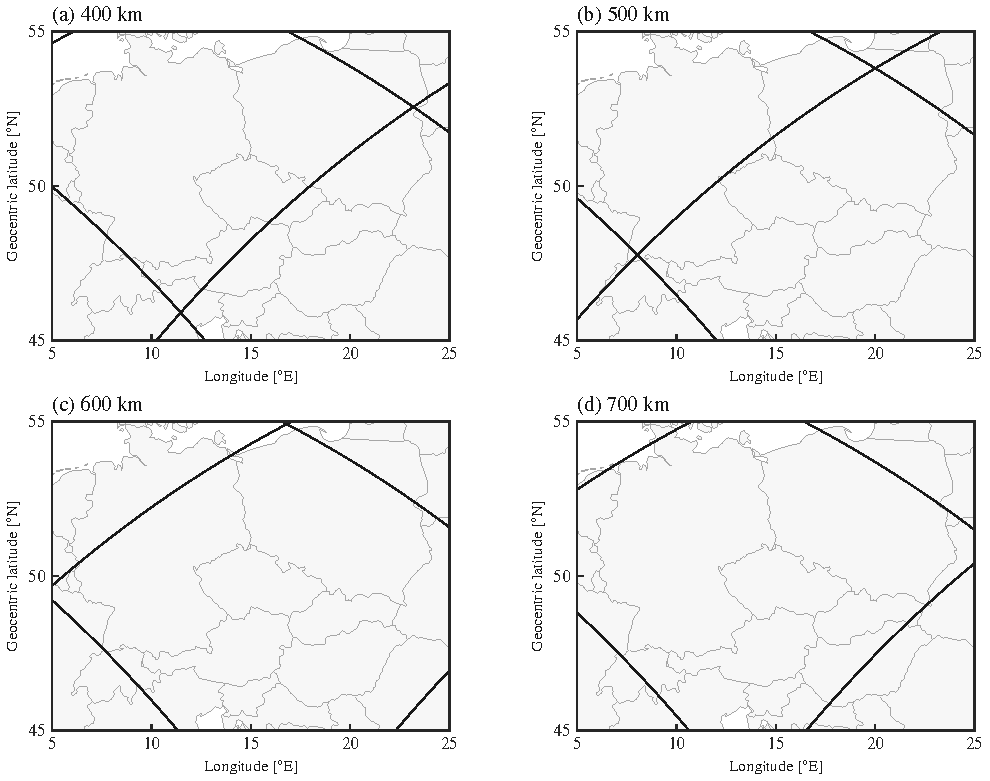
\includegraphics[width=\linewidth,height=0.72\textheight,keepaspectratio]{ground_tracks.pdf}
\caption{First-day subsatellite tracks, shown with geocentric latitude.
Country boundaries provide context; these lines do not indicate the full
sensor footprint. Country boundaries: Natural Earth.}
\label{fig:tracks}
\end{figure}

Figure~\ref{fig:timeline} illustrates the first 72 hours for the grid point
at $14.75^{\circ}$E, $49.75^{\circ}$N. Markers show window centres to keep
short windows visible at this scale; bars retain their sampled durations.
This example is illustrative and is not the 500 km largest-gap target.

\begin{figure}[htbp]
\centering
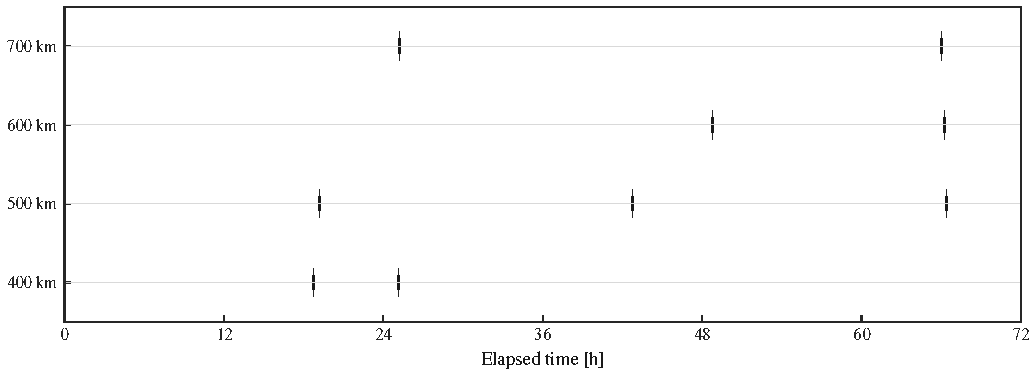
\includegraphics[width=\linewidth]{observation_timeline.pdf}
\caption{Observation windows for an example target during the first
72 hours. Markers indicate window centres; their marker widths do not
represent observation duration.}
\label{fig:timeline}
\end{figure}

\FloatBarrier
\begin{thebibliography}{9}
\bibitem{nag2016}
Nag, S., Hughes, S. P., and Le Moigne, J.,
``Streamlining the Design Tradespace for Earth Imaging Constellations,''
\textit{AIAA SPACE 2016}, 2016.
\url{https://doi.org/10.2514/6.2016-5561}.
\bibitem{hughes2014}
Hughes, S. P., Qureshi, R. H., Cooley, D. S., Parker, J. J. K., and Grubb, T. G.,
``Verification and Validation of the General Mission Analysis Tool (GMAT),''
\textit{AIAA/AAS Astrodynamics Specialist Conference}, 2014.
NASA NTRS Document 20140017798.
\bibitem{nickel2016}
Nickel, C., Lebois, R., Lutz, S., Dichmann, D., and Parker, J.,
``Monte Carlo Analysis as a Trajectory Design Driver for the TESS Mission,''
2016. NASA NTRS Document 20160010500.
\bibitem{wgs84}
National Geospatial-Intelligence Agency,
``World Geodetic System 1984 (WGS 84),'' defining parameters,
\url{https://earth-info.nga.mil/index.php?dir=wgs84&action=wgs84},
accessed 9 November 2026.
\bibitem{naturalearth}
Natural Earth, ``Admin 0 -- Countries, 1:50m,'' public-domain cartographic data,
\url{https://www.naturalearthdata.com/downloads/50m-cultural-vectors/},
accessed 9 November 2026.
\end{thebibliography}
\end{document}
